
\zsavepos{header-1}

\zsavepos{header-1}\section{Introduction\zsavepos{header-2\zsavepos{header-2}}
\zsavepos{header-3}\zlabel{header}
}\zsavepos{header-3}\zlabel{header}

\label{sec:intro}
Procedural graphs, though can intuitively represent the execution of actions for goal achievement~\cite{momouchi1980control, ren2023constructing}, suffer from the high cost of expert-construction~\cite{herbst1999inductive, maqbool2019comprehensive}.
The automatic extraction of procedural graphs from procedural documents thus has huge potential, as it would enable users to easily understand how to logically perform a goal~(e.g, how a restaurant serves the customers) by skimming visual graphs~(e.g., Figure~\ref{fig:task_b} instead of reading lengthy documents~(e.g., Figure~\ref{fig:task_a}).

However, obtaining optimal procedural graphs is not easy --- as shown in Figure~\ref{fig:task_b}, it requires representing not only sequential actions in the procedure~(e.g., \uppercase\expandafter{\romannumeral1}-4  $\rightarrow$ \uppercase\expandafter{\romannumeral1}-5), but also non-sequentially executed actions~(e.g., \uppercase\expandafter{\romannumeral1}-7.1 \& \uppercase\expandafter{\romannumeral1}-7.2]) and vital constraints for the actions~(e.g., C-2).
Off-the-shelf attempts only meet part of the requirements. For example, \citet{bellan2023pet, ren2023constructing} fail to represent ``customers can order only the dishes or drinks, or both''~(\uppercase\expandafter{\romannumeral1}-2.1 \& \uppercase\expandafter{\romannumeral1}-2.2) due to its inherent limitation for representing complex non-sequential actions.
Besides, current solutions only focus on hand-written rules~\cite{sholiq2022generating} or customized networks~\cite{bellan2023pet} on a small group of cherry-picked instances. This brings up the question of \textit{whether the existing studies have well solved the automated extraction of procedural graphs from procedural documents}~(\textit{Q1}). If the answer is ``no'', we are also interested in \textit{whether the emerging large language models~(LLMs) can bring new opportunities to this task}~(\textit{Q2}).

\begin{figure*}[t]
    \zsavepos{figure*-1}
    \zsavepos{figure*-1}
    \centering
    \subfigure[Procedural Graph]{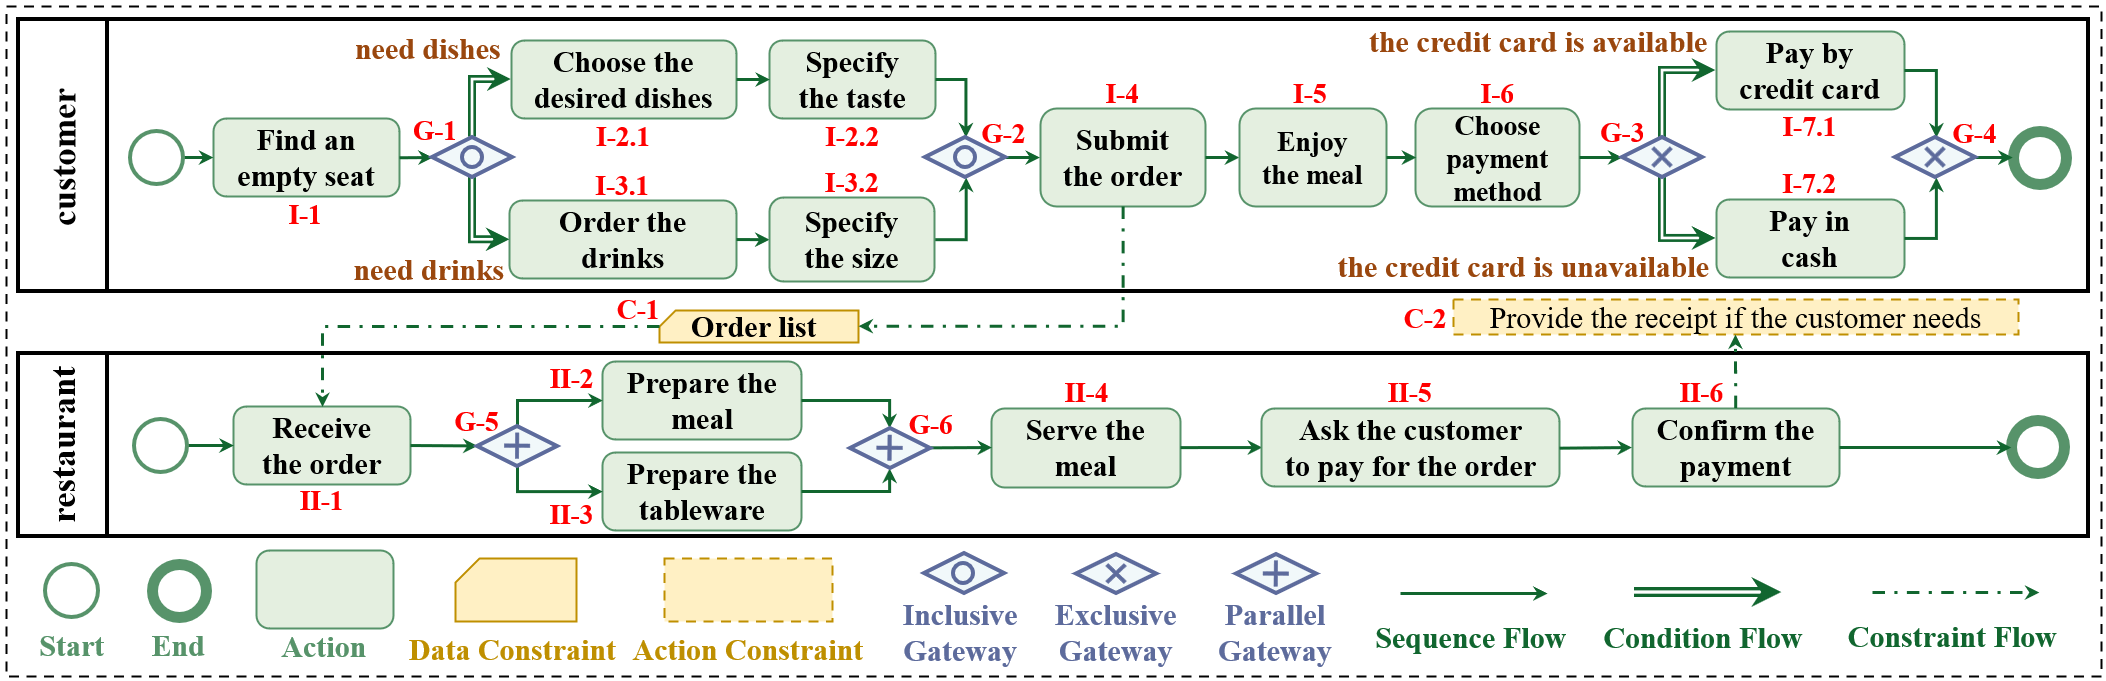
\includegraphics[width=1\textwidth]{figures/Task_b.png}\label{fig:task_b}}\vspace{-5pt}
    \subfigure[Procedural Document]{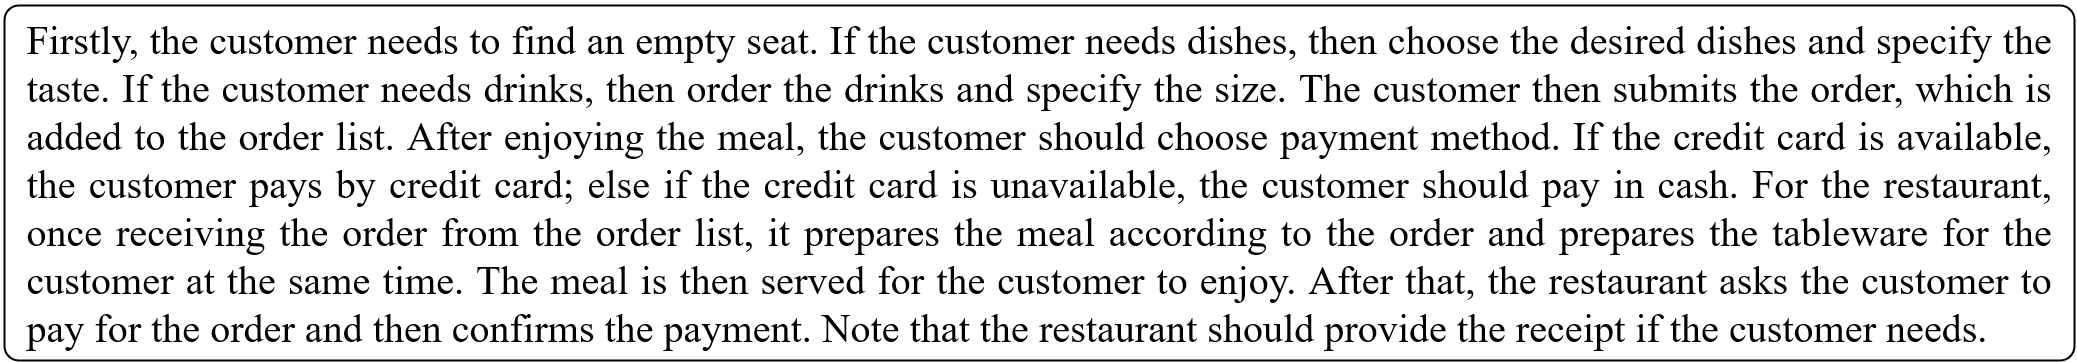
\includegraphics[width=1\textwidth]{figures/Task_a.png}\label{fig:task_a}}

    \zsavepos{figure*-2}

    \zsavepos{figure*-2}
    \zsavepos{figurecap*-1}
    \zsavepos{figurecap*-1}\caption{The procedure of how a restaurant serves the customers in procedural graph~(a) and document~(b).}\zsavepos{figurecap*-2}\zsavepos{figurecap*-2}
    \label{fig:task}
    \zlabel{figure*}

    \zlabel{figure*}
\end{figure*}

To answer \textit{Q1}, we propose to construct a standard benchmark for the \underline{P}rocedur\underline{A}l \underline{G}raphs \underline{E}xtraction from \underline{D}ocuments~(\benchmark). As far as we know, there lack of large-scale datasets of document-graph pairs for training and evaluating optimal procedural graph extraction models~(cf., Table~\ref{datasets}). We want to equip \benchmark with the largest publicly available dataset. Although there exist plenty of procedural documents on the Internet, it is too costly to filter the low-quality ones and annotate optimal procedural graphs matching all requirements. As a remedy, we build the dataset based on a model collection of business process~\cite{dumas2018fundamentals}, which has summarized business processes into high-quality procedural graphs with complete sequential actions, non-sequential actions, and constraints. Thus, constructing procedural document-graph pairs turns into assigning a suitable procedural document to a given procedural graph. We approach it via a three-stage pipeline --- we progressively transfer the structured information on the procedural graph into natural language text, adjust its narration, and improve the coherence and naturalness, finally generating a suitable document. In this way, we develop a dataset with 3,394 high-quality procedural document-graph pairs that are about ten times larger than the previous largest datasets~\cite{ackermann2021data,qian2020approach}. According to the underlying structure of optimal procedural graphs, we introduce {three metrics} to evaluate five state-of-the-art methods~\cite{sonbol2023machine,neuberger2023beyond,sholiq2022generating}.

To further answer \textit{Q2}, we investigate the performance of three advanced LLMs~(Flan-T5~\cite{chung2022scaling}, ChatGPT~\cite{ouyang2022training} and Llama2~\cite{touvron2023llama}) and utilize a self-refine strategy to improve the ability of LLMs. In total, we evaluate ten methods in our \benchmark benchmark. Extensive experiments on our benchmark reveal that existing studies struggle to accurately extract sequential actions, constraints, and organize non-sequential actions of procedural documents. While LLMs have shown significant improvement in sequential action and constraint extraction, they still face challenges with non-sequential action organization. Our detailed analysis of the results leads us to propose improvement strategies to help large language models better understand non-sequential actions and use correct gateways to represent them. We hope \benchmark can be a key milestone for automatic procedural graphs extraction, offering insights into research on logical reasoning among non-sequential elements.
In summary, we highlight \benchmark as follows:
%
\begin{itemize}
    \item We build a novel benchmark named \benchmark, which standardly evaluates the progress of current procedural graphs extraction from documents and explores the potential of emerging LLMs.
    %
    \item We equip \benchmark with the largest procedural document-graph dataset, whose high quality is achieved by a three-stage pipeline and verified via both automatic and human evaluation.
    \item We systematically evaluate state-of-the-art solutions in \benchmark and reveal that they have trouble extracting optimal procedural graphs due to their heavy reliance on hand-written rules and limited available data.
    \item We investigate advanced LLMs in \benchmark and empower them with a self-refine strategy, showing their adavantages in identifying sequential actions and constraints, and pointing out their gaps in building complex logic of graphs.
\end{itemize}
